\documentclass[a4paper,11pt]{article}

\usepackage{amsmath}
\usepackage{amssymb}
\usepackage{amsthm}
\usepackage{graphicx}
\usepackage{enumerate}
\usepackage{booktabs}
%you can add more packages using the same code above

%------------------

\usepackage{hyperref}
\hypersetup{hypertex=true,
colorlinks=true,
linkcolor=black,
anchorcolor=black,
citecolor=black}

%-------------------

%------------------

%Everything before begin document is called the pre-amble and sets out how the document will look
%It is recommended you don't touch the pre-amble until you are familiar with LateX

\begin{document}
	
\title{Introduction to AI Coursework}
\date{}
\maketitle



%The following code is not run because of the percentage sign, but you might find it useful for future work
% \tableofcontents

\section{Anlysis on the Penguin Dataset}

\subsection{EDA on Penguin Datasets}
This dataset comprimises features such as species, island and bill\_length\_mm. Firstly, I conducted an analysis 
to determine the type, number of values, number of unique values, and proportion of missing values for each feature within the dataset. The
anlysis is present in Table 1.

\begin{table}[h]
	\centering
	\caption{Summary of Features}
	\begin{tabular}{lcccc}
		\toprule
		Feature & Type & Count & Nunique & \% Null \\
		\midrule
		species & object & 344 & 3 & 0.000000 \\
		island & object & 344 & 3 & 0.000000 \\
		bill\_length\_mm & float64 & 342 & 164 & 0.581395 \\
		bill\_depth\_mm & float64 & 342 & 80 & 0.581395 \\
		flipper\_length\_mm & float64 & 342 & 55 & 0.581395 \\
		body\_mass\_g & float64 & 342 & 94 & 0.581395 \\
		sex & object & 333 & 2 & 3.197674 \\
		year & int64 & 344 & 3 & 0.000000 \\
		\bottomrule
	\end{tabular}
\end{table}
Obviously, the proportion of missing values is not substantial. Therefore, rows containing missing values will be dropped.
The distribution of numerical features is illustrated in Figure \ref{fig:numerical-features}.

\begin{figure}[htbp]
    \centering
    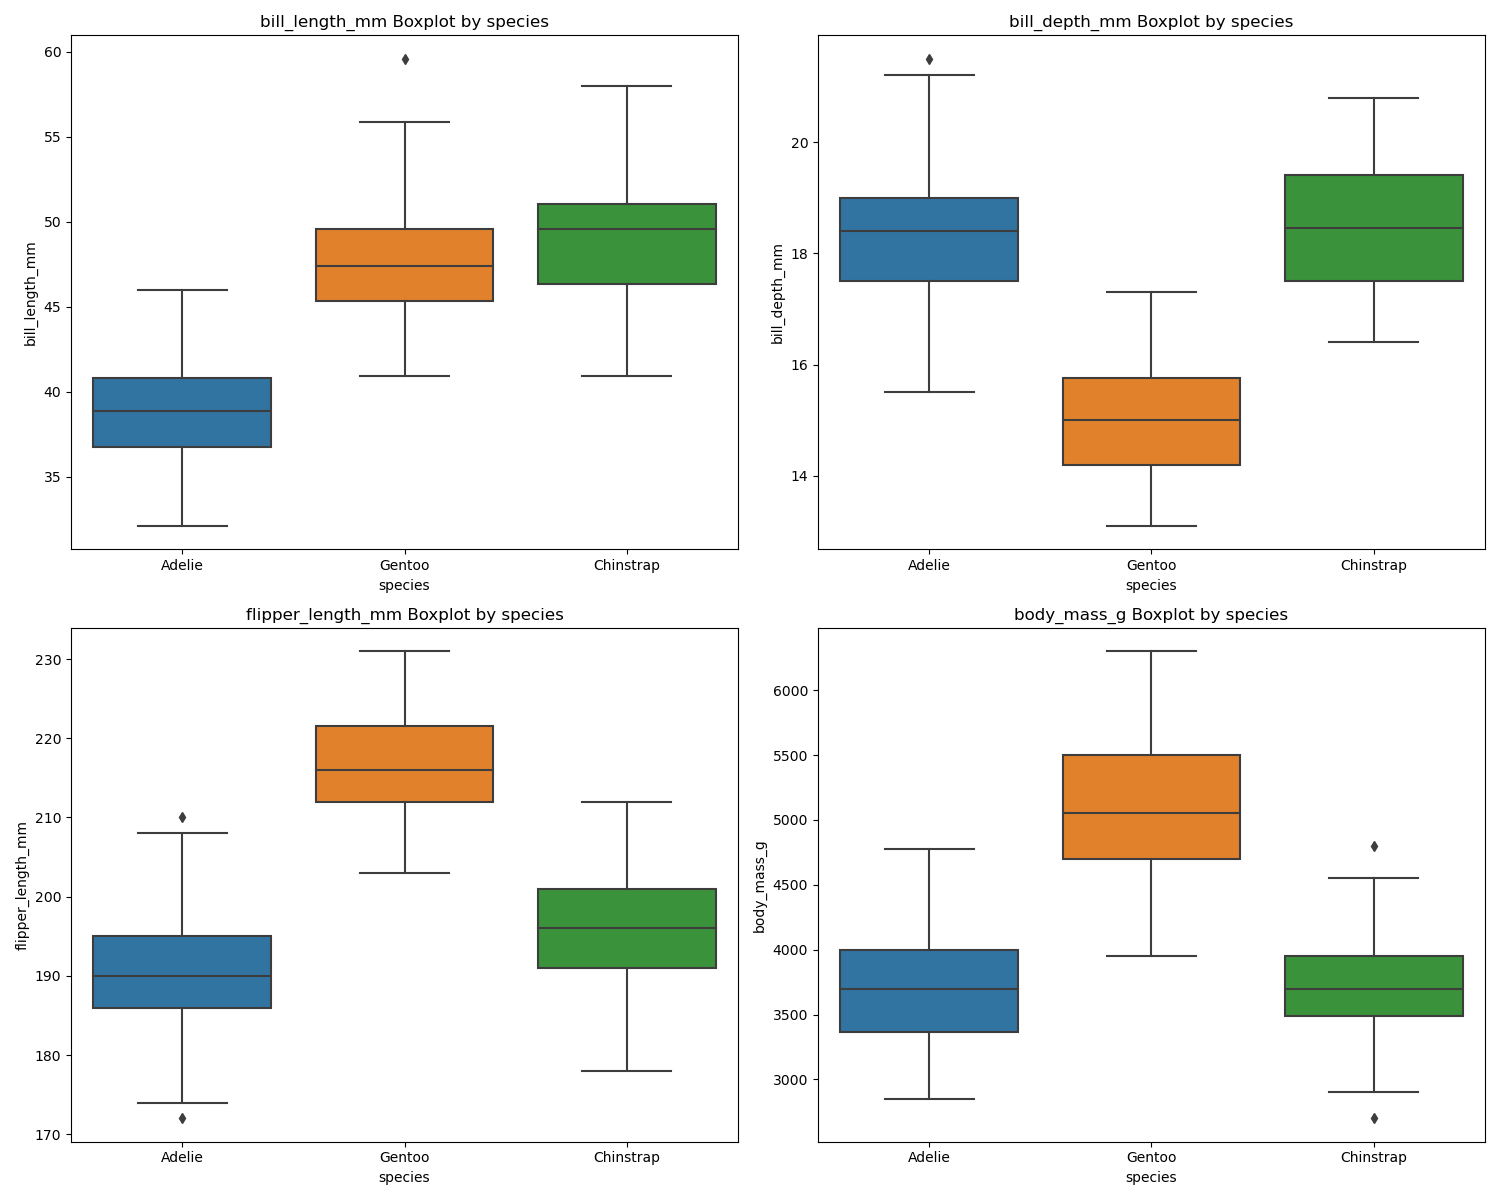
\includegraphics[scale=0.45]{numerical-features}
    \caption{Distribution of different numerical features}
    \label{fig:numerical-features}
\end{figure}
\noindent

\noindent
Subsequently, I employed Cramér's V statistic to measure the correlation between different features and generated a heatmap accordingly.
According to Figure 1, the features sex and year exhibit the quite low correlation with species; hence, these two features 
will not be applied to build the prediction model.


\begin{figure}[htbp]
    \centering
    \includegraphics[scale=0.45]{Cramér-s-V.png}
    \caption{Correlation between different features}
    \label{fig: }
\end{figure}

\subsection{Model Training}

Before building the model, I preprocessed the data based on the previous analysis. Firstly, I dropped the features sex and year. Then, 
I utilised label encoding to encode the categorical feature island and the target feature species. Finally, I split the dataset into 
training and testing sets according to a 4:1 ratio. 

\begin{table}[htbp]
	\centering
	\caption{Best parameters of Decision Tree and Random Forest}
	\begin{tabular}{lcccc}
		\toprule
		& Decision Tree & Random Forest\\
		\midrule
		criterion & entropy &gini \\
		max\_depth & 13 & 12\\
		min\_samples\_split & 13 & 17 \\
		min\_samples\_leaf & 1 & 1 \\
		max\_leaf\_nodes & 32 & 31 \\
        n\_estimators& - & 131 \\
		\bottomrule
	\end{tabular}
\end{table}


\noindent
Criterion represents the criterion for node splitting, max\_depth is the maximum depth of the decision tree,
min\_samples\_split is the minimum number of samples required to split a node, min\_samples\_leaf is the minimum number of samples required to be at a leaf node.
max\_leaf\_nodes is the maximum number of leaf nodes, and n\_estimators is the number of decision tress.


\noindent
The KNN was employed as the baseline model because KNN is a non-parametric and lazy method, meaning that the model does not explicitly 
learn from the data during the training phase. Moreover, I also applied Decision Tree and Random Forest algorithms to 
build two classification models. In this research, optuna was employed for fine-tuning. The monitoring metric for parameter tuning is 
the average accuracy obtained through 5-fold cross-validation. The optimal parameters are determined by the highest average accuracy 
achieved across 50 trials.

\subsection{Results Evaluation}
In this research, the confusion matrix was utilised to evaluate the performance of different models.

\begin{figure}[htbp]
    \centering
    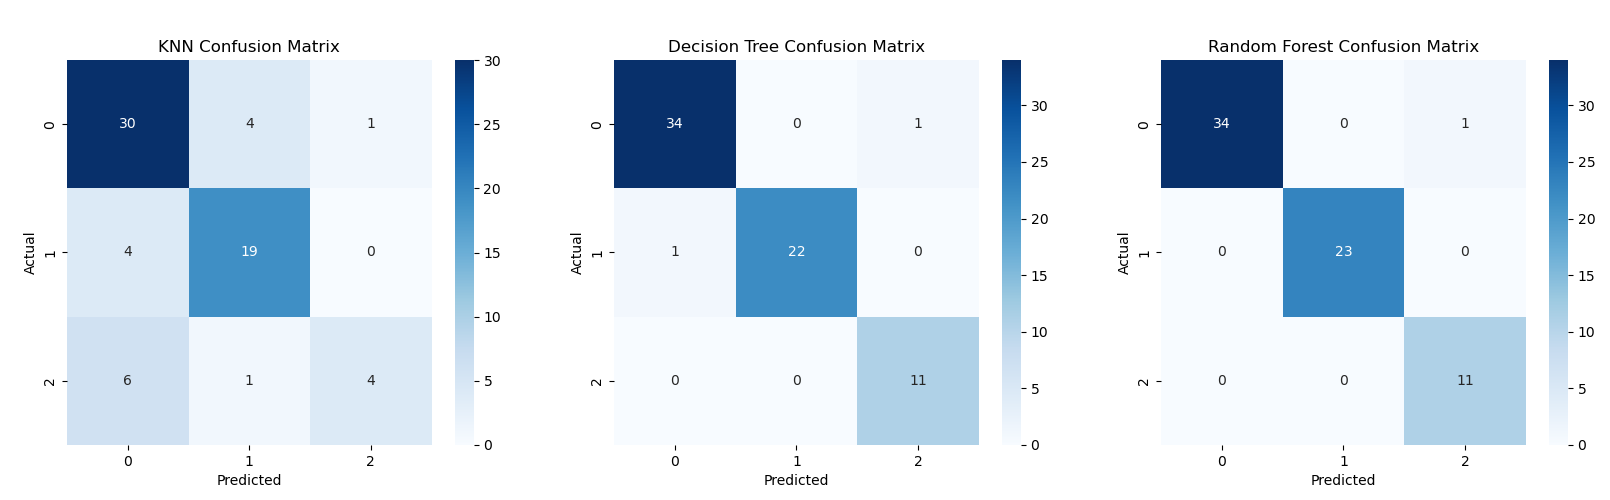
\includegraphics[scale=0.32]{Confusion-Matrix.png}
    \caption{Confusion Matrix}
    \label{fig: }
\end{figure}

\noindent
As shown in Figure 2, both the decision tree and random forest models exhibit higher classification performance compared to KNN. 
The random forest model has only one misclassification, while the decision tree has two misclassifications, and KNN has 20 misclassifications.

\begin{table}[htbp]
	\centering
	\caption{Models' performance on different metrics}
	\begin{tabular}{lcccc}
		\toprule
		&-& KNN & Decision Tree & Random Forest\\
		\midrule
		& accuracy & 0.77 & 0.97 & 0.99\\
        & macro avg precision & 0.78 & 0.96 & 0.97\\
        & macro avg recall & 0.68 & 0.98& 0.99\\
        & macro avg f1-score& 0.70& 0.97& 0.98\\
		\bottomrule
	\end{tabular}
\end{table}

\noindent
In addition, accuracy, macro average precision, macro average recall, and macro average F1-score were employed to evaluate the performance of the models.
As shown in Table 3, he performance of both the decision tree and random forest models surpassed the baseline model KNN across all metrics. Among them, the random forest model exhibited the best classification performance, achieving the highest scores across all metrics.







\section{Challenges in AI}
The advancement of AI technology is gradually reshaping human society. Both the personalised recommendations on video platforms like YouTube 
and the drones employed to execute perilous tasks by are outcomes of AI algorithm applications. Undeniably, AI technology has brought us many conveniences.
However, the application of AI technology also brings forth numerous issues and challenges. As a data-driven technology, undoubtedly, this 
raises concerns regarding data protection.

\noindent
In the 2010s, the Facebook–Cambridge Analytica data scandal that occurred drew widespread public attention. 
Cambridge Analytica utilised user data to target political advertisements without obtaining consent from the users. Finally, Facebook was fined \$5 billion for this incident.
In this incident, the role of the law was primarily punitive after the fact. Indeed, proactive constraints are equally important. Many countries and 
regions around the world have made efforts in this regard, such as the European Union's GDPR. Additionally, companies should fulfill their 
ethical obligations to ensure that users have the right to be informed about and to decide on the usage of their data.

\noindent
The security of AI is also a topic of ongoing public concern. In 2019, a Tesla car owner was charged with manslaughter for 
a fatal traffic accident involving the use of the semi-autonomous driving system Autopilot. Aside from personal safety, AI also has the potential to impact social order. The recent popularity of generative AI also poses the risk of being abused.
For example, in 2023, A fake news video featuring a fabricated speech by Japanese Prime Minister Fumio Kishida, created by an internet user, went viral online, garnering millions of views in a short period. To address the potential risks
associated with AI, the European Union introduced the Artificial Intelligence Act in 2023 to tackle these challenges. According to the AI Act, artificial intelligence systems will be categorized into four different risk levels.
For high-risk artificial intelligence systems, the "Artificial Intelligence Act" establishes a comprehensive lifecycle regulatory framework covering pre-market, in-market, and post-market stages. The implementation of differentiated regulation 
for artificial intelligence systems based on different risk levels provides a potential solution. developers of AI should also uphold 
the most fundamental social responsibility. Moreover, efforts should be made to enhance the robustness and reliability of AI systems, thereby minimizing the risks associated with AI technology as much as possible.

\noindent
In conclusion, to address the challenges posed by AI, it is crucial to enhance legal frameworks, as laws serve as the most robust safeguard for societal order. In addition to legal frameworks, 
Furthermore, AI developers should establish reliable accountability mechanisms to prevent the misuse of data and mitigate the adverse effects of AI systems.












\begin{thebibliography}{99}

\bibitem{lamport94}
  Leslie Lamport,
  \textit{\LaTeX: a document preparation system},
  Addison Wesley, Massachusetts,
  2nd edition,
  1994.
  
\bibitem{referencing}
    Wikibooks,
    \textit{LaTeX/Bibliography Management},
    [0nline],
    Accessed at https://en.wikibooks.org/wiki/LaTeX/Bibliography\_Management,
    (DATE ACCESSED).
    

\end{thebibliography}

\end{document}